\chapter{Hybrid Medical Imaging}
\label{ch:hybrid_imaging}

% Chapter-opening illustrated modality infographic.
\begin{center}
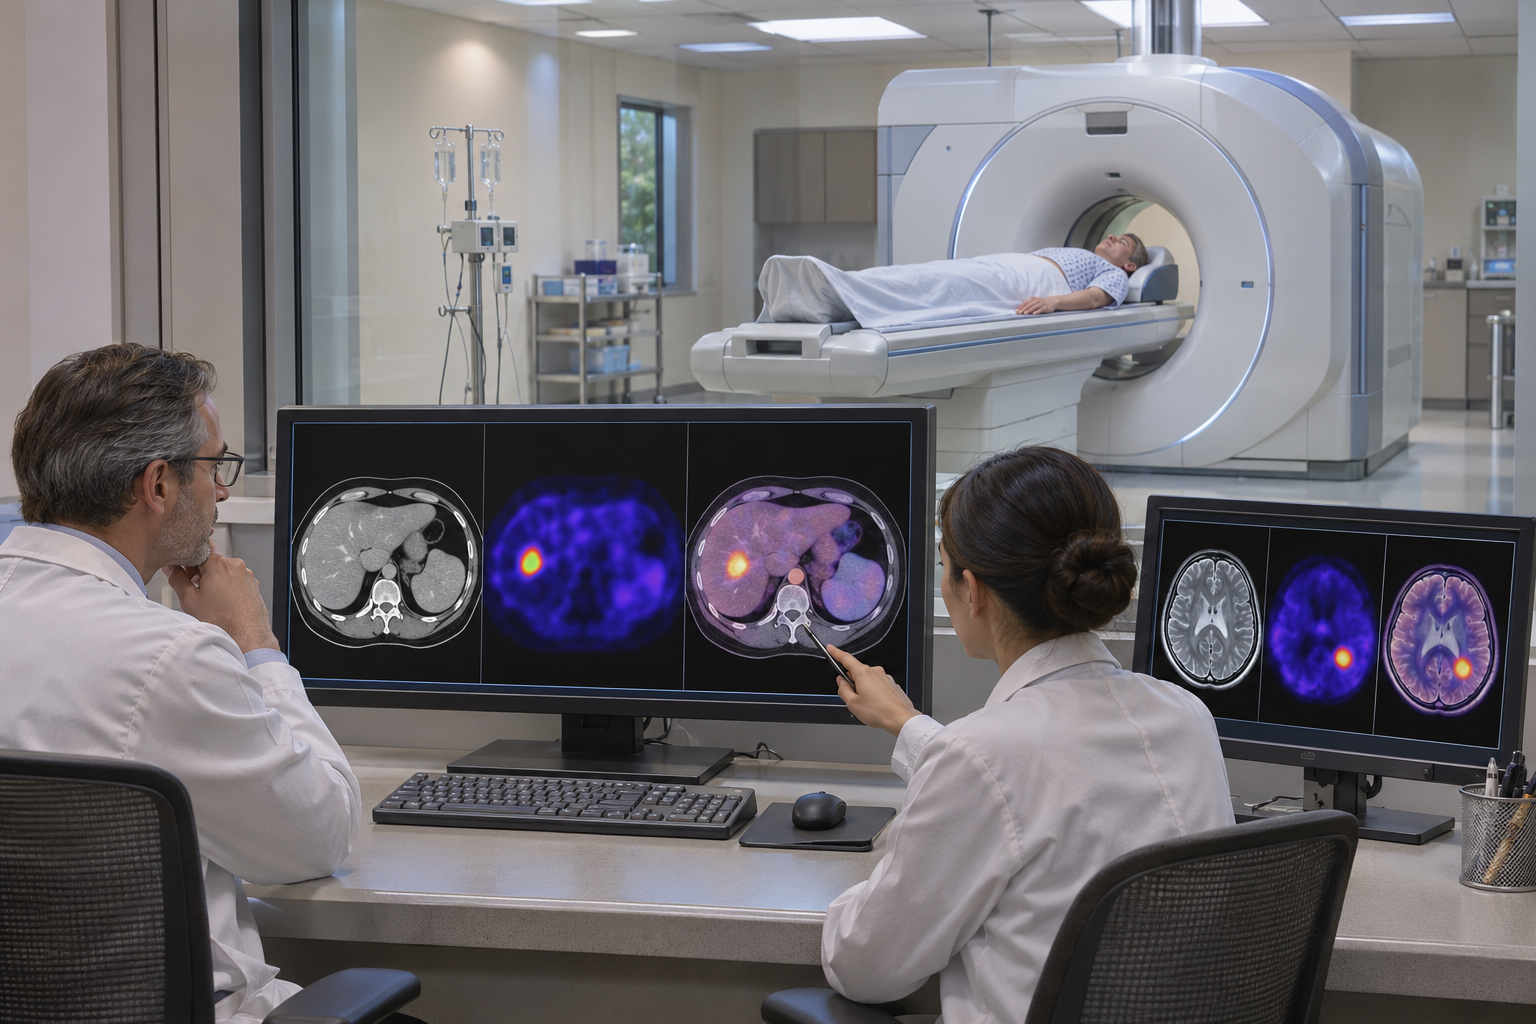
\includegraphics[width=\textwidth,keepaspectratio]{modalities/infographics/hybrid_imaging_realistic.png}
\end{center}
\begin{center}\footnotesize Hybrid imaging registers and combines functional tracer information with anatomical CT or MRI; alignment and the original component images both matter. AI-generated illustration; fused scans are not clinical studies.\end{center}

\section{Overview}
Hybrid imaging combines two or more complementary medical imaging modalities to obtain anatomical, physiological, metabolic, or molecular information within a single examination or a co-registered imaging dataset. Its objective is to address limitations of individual modalities. For example, PET can identify increased metabolic activity but may provide limited anatomical detail, while CT can show the location, dimensions, and morphology of the corresponding lesion.

\begin{center}
\begin{tabular}{@{}p{0.32\textwidth}p{0.22\textwidth}p{0.38\textwidth}@{}}
\toprule
\textbf{Hybrid modality} & \textbf{Anatomical information} & \textbf{Functional or molecular information} \\
\midrule
Fluorescence/X-ray imaging & X-ray & Molecular fluorescence \\
Optical coherence tomography/IVUS & Vascular microstructure & Complementary vascular tissue characterization \\
PET/CT & CT & PET \\
PET/MRI & MRI & PET \\
PET/Ultrasound & Ultrasound & PET \\
Photoacoustic ultrasound & Ultrasound & Optical absorption and tissue oxygenation \\
SPECT/CT & CT & SPECT \\
SPECT/MRI & MRI & SPECT \\
Ultrasound/CT fusion & CT and ultrasound & Real-time ultrasound and Doppler \\
Ultrasound/MRI fusion & MRI and ultrasound & Real-time ultrasound and Doppler \\
\bottomrule
\end{tabular}
\end{center}

PET/CT, PET/MRI, and SPECT/CT are the principal clinically established hybrid imaging modalities. Other combinations are specialized, software-based, or investigational.

The catalogue includes established, supplementary, and investigational applications. Assignments are illustrative rather than formal first-line imaging recommendations. The entries overlap with PET, SPECT, CT, and MRI catalogues and require individual validation against clinical guidance.

\section{Where hybrid imaging is used}
The following examples describe combinations that can add anatomical localization to functional or molecular findings. They do not imply that the listed hybrid examination is always the preferred first-line test.

\subsection{Neurological and neurodegenerative diseases}
\begin{enumerate}[leftmargin=*,itemsep=0.45em,topsep=0.4em]
\item \textbf{Alzheimer disease.} Useful imaging findings include: PET/MRI. Characteristic Imaging Findings: Regional hypometabolism, amyloid deposition and cerebral atrophy.
\item \textbf{Amyotrophic lateral sclerosis.} Useful imaging findings include: PET/MRI. Characteristic Imaging Findings: Reported metabolic and structural motor pathway abnormalities.
\item \textbf{Corticobasal syndrome.} Useful imaging findings include: PET/MRI. Characteristic Imaging Findings: Asymmetric cortical atrophy and hypometabolism.
\item \textbf{Dementia with Lewy bodies.} Useful imaging findings include: PET/MRI. Characteristic Imaging Findings: Occipital hypometabolism with structural assessment.
\item \textbf{Frontotemporal dementia.} Useful imaging findings include: PET/MRI. Characteristic Imaging Findings: Frontal and temporal hypometabolism with corresponding atrophy.
\item \textbf{Huntington disease.} Useful imaging findings include: PET/MRI. Characteristic Imaging Findings: Striatal atrophy and hypometabolism.
\item \textbf{Mild cognitive impairment.} Useful imaging findings include: PET/MRI. Characteristic Imaging Findings: Altered cerebral metabolism or amyloid burden.
\item \textbf{Multiple system atrophy.} Useful imaging findings include: PET/MRI. Characteristic Imaging Findings: Regional hypometabolism and characteristic structural changes.
\item \textbf{Neuroinflammatory disorders.} Useful imaging findings include: PET/MRI. Characteristic Imaging Findings: Molecular tracer abnormalities correlated with structural lesions.
\item \textbf{Parkinson disease.} Useful imaging findings include: SPECT/CT. Characteristic Imaging Findings: Reduced striatal dopamine transporter binding.
\item \textbf{Posterior cortical atrophy.} Useful imaging findings include: PET/MRI. Characteristic Imaging Findings: Posterior cortical hypometabolism and atrophy.
\item \textbf{Primary progressive aphasia.} Useful imaging findings include: PET/MRI. Characteristic Imaging Findings: Regional language network hypometabolism and atrophy.
\item \textbf{Progressive supranuclear palsy.} Useful imaging findings include: PET/MRI. Characteristic Imaging Findings: Midbrain atrophy and regional hypometabolism.
\item \textbf{Vascular dementia.} Useful imaging findings include: PET/MRI. Characteristic Imaging Findings: Regional hypometabolism associated with ischemic lesions.
\end{enumerate}

\subsection{Epilepsy}
\begin{enumerate}[leftmargin=*,itemsep=0.45em,topsep=0.4em]
\item \textbf{Drug-resistant focal epilepsy.} Useful imaging findings include: SPECT/CT, PET/MRI. Characteristic Imaging Findings: Ictal hyperperfusion or interictal hypometabolism.
\item \textbf{Focal cortical dysplasia.} Useful imaging findings include: PET/MRI. Characteristic Imaging Findings: Cortical structural abnormalities and altered metabolism.
\item \textbf{Frontal lobe epilepsy.} Useful imaging findings include: PET/MRI. Characteristic Imaging Findings: Regional frontal hypometabolism.
\item \textbf{Mesial temporal sclerosis.} Useful imaging findings include: PET/MRI. Characteristic Imaging Findings: Hippocampal atrophy, abnormal MRI signal and hypometabolism.
\item \textbf{MRI-negative focal epilepsy.} Useful imaging findings include: PET/MRI. Characteristic Imaging Findings: Regional hypometabolism without obvious structural pathology.
\item \textbf{Occipital lobe epilepsy.} Useful imaging findings include: PET/MRI. Characteristic Imaging Findings: Occipital metabolic abnormalities.
\item \textbf{Parietal lobe epilepsy.} Useful imaging findings include: PET/MRI. Characteristic Imaging Findings: Regional parietal hypometabolism.
\item \textbf{Temporal lobe epilepsy.} Useful imaging findings include: PET/MRI. Characteristic Imaging Findings: Temporal hypometabolism and possible hippocampal sclerosis.
\end{enumerate}

\subsection{Brain tumors}
\begin{enumerate}[leftmargin=*,itemsep=0.45em,topsep=0.4em]
\item \textbf{Astrocytoma.} Useful imaging findings include: PET/MRI. Characteristic Imaging Findings: Variable amino acid uptake and infiltrative MRI abnormalities.
\item \textbf{Brain metastases.} Useful imaging findings include: PET/MRI. Characteristic Imaging Findings: Metabolic abnormalities corresponding to metastatic lesions.
\item \textbf{Ependymoma.} Useful imaging findings include: PET/MRI. Characteristic Imaging Findings: Variable metabolic activity within a structural mass.
\item \textbf{Glioblastoma.} Useful imaging findings include: PET/MRI. Characteristic Imaging Findings: Increased amino acid uptake and infiltrative enhancing mass.
\item \textbf{Medulloblastoma.} Useful imaging findings include: PET/MRI. Characteristic Imaging Findings: Variable metabolic uptake and restricted diffusion.
\item \textbf{Meningioma.} Useful imaging findings include: PET/MRI. Characteristic Imaging Findings: Somatostatin receptor uptake corresponding to a dural mass.
\item \textbf{Oligodendroglioma.} Useful imaging findings include: PET/MRI. Characteristic Imaging Findings: Increased tracer uptake within structurally abnormal tissue.
\item \textbf{Pituitary adenoma.} Useful imaging findings include: PET/MRI. Characteristic Imaging Findings: Focal amino acid tracer uptake within a pituitary lesion.
\item \textbf{Primary CNS lymphoma.} Useful imaging findings include: PET/MRI. Characteristic Imaging Findings: Marked FDG uptake and diffusion restriction.
\item \textbf{Radiation necrosis.} Useful imaging findings include: PET/MRI. Characteristic Imaging Findings: Structural treatment changes with frequently reduced amino acid uptake.
\item \textbf{Recurrent glioma.} Useful imaging findings include: PET/MRI. Characteristic Imaging Findings: Increased amino acid uptake within suspected viable tumor.
\item \textbf{Tumor pseudoprogression.} Useful imaging findings include: PET/MRI. Characteristic Imaging Findings: Variable tracer uptake in treatment-related abnormalities.
\end{enumerate}

\subsection{Cardiovascular diseases}
\begin{enumerate}[leftmargin=*,itemsep=0.45em,topsep=0.4em]
\item \textbf{Cardiac device infection.} Useful imaging findings include: PET/CT. Characteristic Imaging Findings: Abnormal metabolic uptake around implanted devices.
\item \textbf{Cardiac metastases.} Useful imaging findings include: PET/MRI, PET/CT. Characteristic Imaging Findings: Metabolically active myocardial or pericardial lesions.
\item \textbf{Cardiac sarcoidosis.} Useful imaging findings include: PET/MRI, PET/CT. Characteristic Imaging Findings: Focal inflammatory uptake with possible myocardial fibrosis; FDG imaging requires suppression of physiological myocardial uptake.
\item \textbf{Cardiac tumors.} Useful imaging findings include: PET/MRI. Characteristic Imaging Findings: Structural mass with variable metabolic activity.
\item \textbf{Coronary artery disease.} Useful imaging findings include: PET/CT, SPECT/CT. Characteristic Imaging Findings: Myocardial perfusion abnormalities with coronary anatomical information when dedicated CT protocols are used.
\item \textbf{Coronary microvascular dysfunction.} Useful imaging findings include: PET/CT. Characteristic Imaging Findings: Reduced quantitative myocardial flow reserve.
\item \textbf{Dilated cardiomyopathy.} Useful imaging findings include: PET/MRI. Characteristic Imaging Findings: Ventricular dilatation and altered myocardial metabolism.
\item \textbf{Hibernating myocardium.} Useful imaging findings include: PET/MRI, PET/CT. Characteristic Imaging Findings: Reduced perfusion with preserved glucose metabolism.
\item \textbf{Hypertrophic cardiomyopathy.} Useful imaging findings include: PET/MRI. Characteristic Imaging Findings: Myocardial hypertrophy and reduced regional perfusion reserve.
\item \textbf{Ischemic cardiomyopathy.} Useful imaging findings include: PET/MRI. Characteristic Imaging Findings: Perfusion abnormalities and ventricular dysfunction.
\item \textbf{Multivessel coronary artery disease.} Useful imaging findings include: PET/CT. Characteristic Imaging Findings: Reduced absolute myocardial blood flow.
\item \textbf{Myocardial ischemia.} Useful imaging findings include: PET/CT, SPECT/CT. Characteristic Imaging Findings: Reversible myocardial perfusion defects.
\item \textbf{Myocarditis.} Useful imaging findings include: PET/MRI. Characteristic Imaging Findings: Inflammatory uptake and myocardial edema in selected cases.
\item \textbf{Previous myocardial infarction.} Useful imaging findings include: PET/MRI. Characteristic Imaging Findings: Reduced perfusion and myocardial scar.
\item \textbf{Prosthetic valve endocarditis.} Useful imaging findings include: PET/CT, SPECT/CT. Characteristic Imaging Findings: Abnormal inflammatory or leukocyte uptake around prosthetic valves.
\item \textbf{Transthyretin cardiac amyloidosis.} Useful imaging findings include: SPECT/CT. Characteristic Imaging Findings: Myocardial bone-tracer uptake confirmed on SPECT and interpreted with validated criteria.
\end{enumerate}

Bone-tracer uptake alone does not establish ATTR cardiac amyloidosis. Interpretation requires appropriate clinical criteria and evaluation for a monoclonal protein to avoid misclassifying AL amyloidosis.

\subsection{Vascular diseases}
\begin{enumerate}[leftmargin=*,itemsep=0.45em,topsep=0.4em]
\item \textbf{Active vascular microcalcification.} Useful imaging findings include: PET/CT. Characteristic Imaging Findings: Increased ¹⁸F-NaF uptake within vascular plaques.
\item \textbf{Aortitis.} Useful imaging findings include: PET/CT. Characteristic Imaging Findings: Increased aortic wall uptake.
\item \textbf{Atherosclerosis.} Useful imaging findings include: PET/CT. Characteristic Imaging Findings: Plaque-associated inflammatory activity.
\item \textbf{Carotid plaque inflammation.} Useful imaging findings include: PET/MRI. Characteristic Imaging Findings: Plaque morphology and inflammatory metabolic activity.
\item \textbf{Giant cell arteritis.} Useful imaging findings include: PET/CT. Characteristic Imaging Findings: Increased metabolic activity along large arterial walls.
\item \textbf{Infected aortic aneurysm.} Useful imaging findings include: PET/CT. Characteristic Imaging Findings: Aneurysmal morphology with inflammatory uptake.
\item \textbf{Inflammatory abdominal aortic aneurysm.} Useful imaging findings include: PET/CT. Characteristic Imaging Findings: Periaortic inflammatory metabolic activity.
\item \textbf{Moyamoya disease.} Useful imaging findings include: PET/MRI. Characteristic Imaging Findings: Impaired cerebral perfusion associated with vascular abnormalities.
\item \textbf{Takayasu arteritis.} Useful imaging findings include: PET/CT, PET/MRI. Characteristic Imaging Findings: Arterial wall inflammation and structural vascular abnormalities.
\item \textbf{Vascular graft infection.} Useful imaging findings include: PET/CT, SPECT/CT. Characteristic Imaging Findings: Abnormal tracer accumulation around vascular prostheses.
\end{enumerate}
Several vascular molecular imaging applications remain investigational.

\subsection{Pulmonary and thoracic diseases}
\begin{enumerate}[leftmargin=*,itemsep=0.45em,topsep=0.4em]
\item \textbf{Acute pulmonary embolism.} Useful imaging findings include: V/Q SPECT/CT. Characteristic Imaging Findings: Segmental ventilation-perfusion mismatch.
\item \textbf{Bronchial carcinoid.} Useful imaging findings include: PET/CT. Characteristic Imaging Findings: Somatostatin receptor-positive pulmonary lesion.
\item \textbf{Chronic obstructive pulmonary disease.} Useful imaging findings include: SPECT/CT. Characteristic Imaging Findings: Regional ventilation and perfusion abnormalities.
\item \textbf{Chronic thromboembolic pulmonary hypertension.} Useful imaging findings include: V/Q SPECT/CT. Characteristic Imaging Findings: Persistent mismatched perfusion defects.
\item \textbf{Malignant pleural mesothelioma.} Useful imaging findings include: PET/CT. Characteristic Imaging Findings: Pleural thickening with increased metabolic activity.
\item \textbf{Non-small cell lung carcinoma.} Useful imaging findings include: PET/CT. Characteristic Imaging Findings: Hypermetabolic pulmonary mass and possible metastatic lesions.
\item \textbf{Pulmonary adenocarcinoma.} Useful imaging findings include: PET/CT. Characteristic Imaging Findings: Pulmonary lesion with variable FDG uptake.
\item \textbf{Pulmonary fibrosis.} Useful imaging findings include: PET/CT (investigational). Characteristic Imaging Findings: Variable FDG uptake reported in research; PET/CT is not a routine test to diagnose pulmonary fibrosis.
\item \textbf{Pulmonary metastases.} Useful imaging findings include: PET/CT. Characteristic Imaging Findings: Structural pulmonary nodules with variable metabolic uptake.
\item \textbf{Pulmonary sarcoidosis.} Useful imaging findings include: PET/CT. Characteristic Imaging Findings: Metabolically active pulmonary and nodal granulomatous lesions.
\item \textbf{Pulmonary squamous cell carcinoma.} Useful imaging findings include: PET/CT. Characteristic Imaging Findings: Frequently intense uptake within a pulmonary mass.
\item \textbf{Pulmonary tuberculosis.} Useful imaging findings include: PET/CT. Characteristic Imaging Findings: Structural pulmonary abnormalities with inflammatory uptake.
\item \textbf{Small cell lung carcinoma.} Useful imaging findings include: PET/CT. Characteristic Imaging Findings: Metabolically active primary and metastatic disease.
\item \textbf{Solitary pulmonary nodule.} Useful imaging findings include: PET/CT. Characteristic Imaging Findings: Anatomical nodule with variable metabolic activity.
\item \textbf{Thymic carcinoma.} Useful imaging findings include: PET/CT. Characteristic Imaging Findings: Frequently hypermetabolic mediastinal mass.
\item \textbf{Thymoma.} Useful imaging findings include: PET/CT. Characteristic Imaging Findings: Anterior mediastinal mass with variable uptake.
\end{enumerate}

\subsection{Head and neck diseases}
\begin{enumerate}[leftmargin=*,itemsep=0.45em,topsep=0.4em]
\item \textbf{Adenoid cystic carcinoma.} Useful imaging findings include: PET/MRI. Characteristic Imaging Findings: Variable metabolic uptake and possible perineural extension on MRI.
\item \textbf{Cervical lymph node metastases.} Useful imaging findings include: PET/CT. Characteristic Imaging Findings: Hypermetabolic cervical lymph nodes.
\item \textbf{Esthesioneuroblastoma.} Useful imaging findings include: PET/CT, PET/MRI. Characteristic Imaging Findings: Metabolic or receptor-specific uptake within a sinonasal mass.
\item \textbf{Hypopharyngeal carcinoma.} Useful imaging findings include: PET/CT. Characteristic Imaging Findings: Hypermetabolic primary lesion.
\item \textbf{Laryngeal carcinoma.} Useful imaging findings include: PET/CT. Characteristic Imaging Findings: Increased metabolic uptake within a laryngeal mass.
\item \textbf{Nasopharyngeal carcinoma.} Useful imaging findings include: PET/MRI. Characteristic Imaging Findings: Metabolic abnormalities with skull base and soft-tissue assessment.
\item \textbf{Occult head and neck primary tumor.} Useful imaging findings include: PET/CT. Characteristic Imaging Findings: Potential localization of an otherwise unidentified primary malignancy.
\item \textbf{Oral squamous cell carcinoma.} Useful imaging findings include: PET/CT. Characteristic Imaging Findings: Hypermetabolic primary lesion and possible nodal involvement.
\item \textbf{Oropharyngeal carcinoma.} Useful imaging findings include: PET/CT. Characteristic Imaging Findings: Increased primary and nodal metabolic uptake.
\item \textbf{Salivary gland carcinoma.} Useful imaging findings include: PET/MRI. Characteristic Imaging Findings: Variable metabolic activity within a glandular mass.
\item \textbf{Sinonasal carcinoma.} Useful imaging findings include: PET/MRI. Characteristic Imaging Findings: Metabolic activity with detailed anatomical extension.
\item \textbf{Tongue carcinoma.} Useful imaging findings include: PET/MRI. Characteristic Imaging Findings: Metabolic activity with detailed soft-tissue extension.
\end{enumerate}

\subsection{Thyroid and parathyroid diseases}
\begin{enumerate}[leftmargin=*,itemsep=0.45em,topsep=0.4em]
\item \textbf{Anaplastic thyroid carcinoma.} Useful imaging findings include: PET/CT. Characteristic Imaging Findings: Intense metabolic activity within an aggressive mass.
\item \textbf{Ectopic parathyroid adenoma.} Useful imaging findings include: SPECT/CT, PET/CT. Characteristic Imaging Findings: Focal tracer accumulation at an abnormal anatomical location.
\item \textbf{Ectopic thyroid tissue.} Useful imaging findings include: SPECT/CT. Characteristic Imaging Findings: Anatomical localization of functioning thyroid tissue.
\item \textbf{Follicular thyroid carcinoma.} Useful imaging findings include: SPECT/CT. Characteristic Imaging Findings: Radioiodine-avid metastatic lesions.
\item \textbf{Medullary thyroid carcinoma.} Useful imaging findings include: PET/CT. Characteristic Imaging Findings: Amino acid or metabolic tracer uptake.
\item \textbf{Papillary thyroid carcinoma.} Useful imaging findings include: SPECT/CT. Characteristic Imaging Findings: Localization of radioiodine-avid residual or metastatic tissue.
\item \textbf{Parathyroid adenoma.} Useful imaging findings include: SPECT/CT. Characteristic Imaging Findings: Persistent sestamibi uptake localized to a parathyroid lesion.
\item \textbf{Parathyroid hyperplasia.} Useful imaging findings include: SPECT/CT. Characteristic Imaging Findings: Tracer uptake in hyperfunctioning glands.
\item \textbf{Radioiodine-refractory thyroid carcinoma.} Useful imaging findings include: PET/CT. Characteristic Imaging Findings: Hypermetabolic non-iodine-avid tumor lesions.
\item \textbf{Recurrent hyperparathyroidism.} Useful imaging findings include: PET/CT. Characteristic Imaging Findings: Fluorocholine uptake in residual hyperfunctioning tissue.
\end{enumerate}

\subsection{Breast diseases}
\begin{enumerate}[leftmargin=*,itemsep=0.45em,topsep=0.4em]
\item \textbf{Breast cancer sentinel node localization.} Useful imaging findings include: SPECT/CT (selected adjunct). Characteristic Imaging Findings: SPECT/CT can localize nodes when planar lymphoscintigraphy is inadequate or drainage is anatomically complex.
\item \textbf{HER2-positive breast cancer.} Useful imaging findings include: PET/CT. Characteristic Imaging Findings: Variable tumor metabolic activity.
\item \textbf{Inflammatory breast cancer.} Useful imaging findings include: PET/CT. Characteristic Imaging Findings: Diffuse breast and cutaneous metabolic abnormalities.
\item \textbf{Invasive ductal carcinoma.} Useful imaging findings include: PET/CT, PET/MRI. Characteristic Imaging Findings: Increased metabolic uptake and structural breast lesion.
\item \textbf{Invasive lobular carcinoma.} Useful imaging findings include: PET/MRI. Characteristic Imaging Findings: Infiltrative MRI abnormalities with variable metabolic uptake.
\item \textbf{Metastatic breast carcinoma.} Useful imaging findings include: PET/CT. Characteristic Imaging Findings: Metabolically active distant lesions.
\item \textbf{Multifocal breast carcinoma.} Useful imaging findings include: PET/MRI. Characteristic Imaging Findings: Multiple anatomical and metabolically abnormal lesions.
\item \textbf{Recurrent breast carcinoma.} Useful imaging findings include: PET/CT. Characteristic Imaging Findings: Metabolic activity within suspected recurrent disease.
\item \textbf{Recurrent or metastatic breast cancer with uncertain estrogen receptor status.} Useful imaging findings include: FES PET/CT (selected use). Characteristic Imaging Findings: May detect ER-positive lesions as an adjunct to biopsy; not a general breast cancer test.
\item \textbf{Triple-negative breast cancer.} Useful imaging findings include: PET/CT. Characteristic Imaging Findings: Frequently increased glucose metabolism.
\end{enumerate}

\subsection{Hematological malignancies}
\begin{enumerate}[leftmargin=*,itemsep=0.45em,topsep=0.4em]
\item \textbf{Anaplastic large cell lymphoma.} Useful imaging findings include: PET/CT. Characteristic Imaging Findings: Metabolically active nodal and extranodal disease.
\item \textbf{Burkitt lymphoma.} Useful imaging findings include: PET/CT. Characteristic Imaging Findings: Markedly hypermetabolic tumor masses.
\item \textbf{Diffuse large B-cell lymphoma.} Useful imaging findings include: PET/CT. Characteristic Imaging Findings: Intense metabolic uptake within lymphoma lesions.
\item \textbf{Extramedullary plasmacytoma.} Useful imaging findings include: PET/CT. Characteristic Imaging Findings: Hypermetabolic soft-tissue mass.
\item \textbf{Follicular lymphoma.} Useful imaging findings include: PET/CT. Characteristic Imaging Findings: Metabolically active lymphadenopathy.
\item \textbf{Hodgkin lymphoma.} Useful imaging findings include: PET/CT. Characteristic Imaging Findings: Hypermetabolic nodal and extranodal disease.
\item \textbf{Mantle cell lymphoma.} Useful imaging findings include: PET/CT. Characteristic Imaging Findings: Variable metabolic nodal and extranodal involvement.
\item \textbf{Marginal zone lymphoma.} Useful imaging findings include: PET/CT. Characteristic Imaging Findings: Variable metabolic activity.
\item \textbf{Multiple myeloma.} Useful imaging findings include: PET/CT, PET/MRI. Characteristic Imaging Findings: Metabolically active skeletal and marrow lesions.
\item \textbf{Myeloid sarcoma.} Useful imaging findings include: PET/CT. Characteristic Imaging Findings: Metabolically active extramedullary tumor.
\item \textbf{Peripheral T-cell lymphoma.} Useful imaging findings include: PET/CT. Characteristic Imaging Findings: Increased metabolic uptake.
\item \textbf{Primary mediastinal B-cell lymphoma.} Useful imaging findings include: PET/CT. Characteristic Imaging Findings: Hypermetabolic mediastinal mass.
\item \textbf{Richter transformation.} Useful imaging findings include: PET/CT. Characteristic Imaging Findings: Intensely metabolically active suspicious lesions.
\item \textbf{Solitary plasmacytoma.} Useful imaging findings include: PET/CT. Characteristic Imaging Findings: Focal metabolically active plasma cell lesion.
\end{enumerate}

\subsection{Gastrointestinal malignancies}
\begin{enumerate}[leftmargin=*,itemsep=0.45em,topsep=0.4em]
\item \textbf{Anal squamous cell carcinoma.} Useful imaging findings include: PET/CT. Characteristic Imaging Findings: Hypermetabolic primary and nodal lesions.
\item \textbf{Appendiceal carcinoma.} Useful imaging findings include: PET/CT. Characteristic Imaging Findings: Variable metabolic activity.
\item \textbf{Colorectal carcinoma.} Useful imaging findings include: PET/CT. Characteristic Imaging Findings: Hypermetabolic primary or metastatic lesions.
\item \textbf{Esophageal carcinoma.} Useful imaging findings include: PET/CT. Characteristic Imaging Findings: Hypermetabolic esophageal mass and metastatic involvement.
\item \textbf{Gastric carcinoma.} Useful imaging findings include: PET/CT. Characteristic Imaging Findings: Variable metabolic uptake within gastric lesions.
\item \textbf{Gastrointestinal lymphoma.} Useful imaging findings include: PET/CT. Characteristic Imaging Findings: Metabolically active intestinal wall abnormalities.
\item \textbf{Gastrointestinal stromal tumor.} Useful imaging findings include: PET/CT. Characteristic Imaging Findings: Metabolic activity within viable tumor.
\item \textbf{Peritoneal carcinomatosis.} Useful imaging findings include: PET/CT, PET/MRI. Characteristic Imaging Findings: Metabolically active peritoneal deposits.
\item \textbf{Rectal carcinoma.} Useful imaging findings include: PET/MRI. Characteristic Imaging Findings: Tumor metabolism with detailed local anatomical assessment.
\item \textbf{Recurrent colorectal carcinoma.} Useful imaging findings include: PET/CT. Characteristic Imaging Findings: Abnormal metabolic uptake within recurrent lesions.
\item \textbf{Recurrent rectal carcinoma.} Useful imaging findings include: PET/MRI. Characteristic Imaging Findings: Metabolic abnormalities correlated with pelvic soft-tissue changes.
\item \textbf{Small bowel adenocarcinoma.} Useful imaging findings include: PET/CT. Characteristic Imaging Findings: Focal metabolically active intestinal mass.
\end{enumerate}

\subsection{Liver, biliary and pancreatic diseases}
\begin{enumerate}[leftmargin=*,itemsep=0.45em,topsep=0.4em]
\item \textbf{Extrahepatic cholangiocarcinoma.} Useful imaging findings include: PET/CT. Characteristic Imaging Findings: Abnormal biliary tumor uptake.
\item \textbf{Focal nodular hyperplasia.} Useful imaging findings include: SPECT/CT. Characteristic Imaging Findings: Preserved or increased colloid uptake in selected lesions.
\item \textbf{Gallbladder carcinoma.} Useful imaging findings include: PET/CT. Characteristic Imaging Findings: Hypermetabolic gallbladder mass.
\item \textbf{Hepatic hemangioma.} Useful imaging findings include: SPECT/CT. Characteristic Imaging Findings: Delayed blood-pool tracer accumulation.
\item \textbf{Hepatic metastases.} Useful imaging findings include: PET/MRI. Characteristic Imaging Findings: Metabolic abnormalities with high-resolution liver imaging.
\item \textbf{Hepatic neuroendocrine metastases.} Useful imaging findings include: PET/MRI. Characteristic Imaging Findings: Receptor-specific uptake within hepatic lesions.
\item \textbf{Hepatocellular carcinoma.} Useful imaging findings include: PET/MRI. Characteristic Imaging Findings: Characteristic MRI enhancement with variable metabolic uptake.
\item \textbf{Intrahepatic cholangiocarcinoma.} Useful imaging findings include: PET/CT, PET/MRI. Characteristic Imaging Findings: Metabolically active hepatic mass.
\item \textbf{Pancreatic adenocarcinoma.} Useful imaging findings include: PET/CT. Characteristic Imaging Findings: Hypermetabolic pancreatic mass.
\item \textbf{Pancreatic neuroendocrine tumor.} Useful imaging findings include: PET/CT, PET/MRI. Characteristic Imaging Findings: Somatostatin receptor-positive pancreatic lesion.
\item \textbf{Postoperative bile leak.} Useful imaging findings include: SPECT/CT. Characteristic Imaging Findings: Anatomical localization of extraluminal biliary tracer.
\item \textbf{Recurrent pancreatic carcinoma.} Useful imaging findings include: PET/CT. Characteristic Imaging Findings: Metabolic uptake at suspected recurrence sites.
\end{enumerate}

\subsection{Neuroendocrine and adrenal tumors}
\begin{enumerate}[leftmargin=*,itemsep=0.45em,topsep=0.4em]
\item \textbf{Adrenocortical carcinoma.} Useful imaging findings include: PET/CT. Characteristic Imaging Findings: Metabolically active adrenal mass.
\item \textbf{Gastrinoma.} Useful imaging findings include: PET/CT. Characteristic Imaging Findings: Somatostatin receptor-positive tumor.
\item \textbf{Gastroenteropancreatic neuroendocrine tumor.} Useful imaging findings include: PET/CT. Characteristic Imaging Findings: Somatostatin receptor-positive lesions.
\item \textbf{Glucagonoma.} Useful imaging findings include: PET/CT. Characteristic Imaging Findings: Receptor-specific pancreatic tumor uptake.
\item \textbf{Insulinoma.} Useful imaging findings include: PET/CT, PET/MRI. Characteristic Imaging Findings: GLP-1 receptor-specific uptake in selected tumors.
\item \textbf{Merkel cell carcinoma.} Useful imaging findings include: PET/CT. Characteristic Imaging Findings: Hypermetabolic primary or metastatic lesions.
\item \textbf{Neuroblastoma.} Useful imaging findings include: SPECT/CT. Characteristic Imaging Findings: MIBG-avid primary and metastatic lesions.
\item \textbf{Paraganglioma.} Useful imaging findings include: PET/CT. Characteristic Imaging Findings: Frequently intense somatostatin receptor uptake.
\item \textbf{Pheochromocytoma.} Useful imaging findings include: PET/CT, SPECT/CT. Characteristic Imaging Findings: Receptor-specific or MIBG uptake within adrenal lesions.
\item \textbf{Poorly differentiated neuroendocrine carcinoma.} Useful imaging findings include: PET/CT. Characteristic Imaging Findings: Frequently intense FDG uptake.
\item \textbf{Small bowel neuroendocrine tumor.} Useful imaging findings include: PET/CT. Characteristic Imaging Findings: Receptor-positive intestinal and metastatic lesions.
\item \textbf{VIPoma.} Useful imaging findings include: PET/CT. Characteristic Imaging Findings: Increased receptor-specific uptake.
\item \textbf{Well-differentiated neuroendocrine tumor.} Useful imaging findings include: PET/CT. Characteristic Imaging Findings: Increased receptor-specific tracer uptake.
\end{enumerate}

\subsection{Male reproductive and urinary diseases}
\begin{enumerate}[leftmargin=*,itemsep=0.45em,topsep=0.4em]
\item \textbf{Bladder carcinoma.} Useful imaging findings include: PET/CT. Characteristic Imaging Findings: Metabolic uptake in selected primary or metastatic lesions.
\item \textbf{Metastatic castration-resistant prostate cancer.} Useful imaging findings include: PSMA PET/CT. Characteristic Imaging Findings: Variable PSMA expression across metastatic lesions.
\item \textbf{Neuroendocrine prostate carcinoma.} Useful imaging findings include: FDG PET/CT. Characteristic Imaging Findings: Increased glucose metabolism with potentially reduced PSMA uptake.
\item \textbf{Penile carcinoma.} Useful imaging findings include: PET/CT. Characteristic Imaging Findings: Metabolically active primary or nodal lesions.
\item \textbf{Prostate adenocarcinoma.} Useful imaging findings include: PSMA PET/CT, PET/MRI. Characteristic Imaging Findings: Increased PSMA uptake within primary or metastatic lesions.
\item \textbf{Prostate lesion requiring targeted biopsy.} Useful imaging findings include: MRI/Ultrasound fusion. Characteristic Imaging Findings: MRI-defined suspicious lesion localized using real-time ultrasound.
\item \textbf{Recurrent prostate carcinoma.} Useful imaging findings include: PSMA PET/CT. Characteristic Imaging Findings: Localization of recurrent or metastatic disease.
\item \textbf{Renal cell carcinoma.} Useful imaging findings include: PET/CT. Characteristic Imaging Findings: Variable metabolic activity within metastatic lesions.
\item \textbf{Renal lymphoma.} Useful imaging findings include: PET/CT. Characteristic Imaging Findings: Hypermetabolic renal lesions.
\item \textbf{Testicular seminoma.} Useful imaging findings include: PET/CT. Characteristic Imaging Findings: Metabolic activity within selected residual masses.
\end{enumerate}

\subsection{Female reproductive diseases}
\begin{enumerate}[leftmargin=*,itemsep=0.45em,topsep=0.4em]
\item \textbf{Cervical carcinoma.} Useful imaging findings include: PET/MRI. Characteristic Imaging Findings: Metabolic activity with detailed parametrial and pelvic anatomy.
\item \textbf{Endometrial carcinoma.} Useful imaging findings include: PET/MRI. Characteristic Imaging Findings: Metabolic tumor activity and myometrial invasion assessment.
\item \textbf{Endometrial stromal sarcoma.} Useful imaging findings include: PET/MRI. Characteristic Imaging Findings: Variable metabolic activity within a uterine lesion.
\item \textbf{Fallopian tube carcinoma.} Useful imaging findings include: PET/CT. Characteristic Imaging Findings: Metabolically active adnexal or metastatic lesions.
\item \textbf{Ovarian carcinoma.} Useful imaging findings include: PET/CT, PET/MRI. Characteristic Imaging Findings: Metabolically active pelvic and peritoneal lesions.
\item \textbf{Primary peritoneal carcinoma.} Useful imaging findings include: PET/CT. Characteristic Imaging Findings: Hypermetabolic peritoneal deposits.
\item \textbf{Recurrent ovarian carcinoma.} Useful imaging findings include: PET/CT. Characteristic Imaging Findings: Metabolic uptake within recurrent lesions.
\item \textbf{Uterine leiomyosarcoma.} Useful imaging findings include: PET/MRI. Characteristic Imaging Findings: Metabolic activity within a heterogeneous uterine mass.
\item \textbf{Vaginal carcinoma.} Useful imaging findings include: PET/MRI. Characteristic Imaging Findings: Metabolic uptake with local soft-tissue characterization.
\item \textbf{Vulvar carcinoma.} Useful imaging findings include: PET/CT. Characteristic Imaging Findings: Metabolically active primary and nodal lesions.
\end{enumerate}

\subsection{Bone and skeletal diseases}
\begin{enumerate}[leftmargin=*,itemsep=0.45em,topsep=0.4em]
\item \textbf{Bone lymphoma.} Useful imaging findings include: PET/CT. Characteristic Imaging Findings: Hypermetabolic bone or marrow lesions.
\item \textbf{Chondrosarcoma.} Useful imaging findings include: PET/CT. Characteristic Imaging Findings: Variable tumor metabolism.
\item \textbf{Ewing sarcoma.} Useful imaging findings include: PET/CT. Characteristic Imaging Findings: Increased metabolic activity within a skeletal mass.
\item \textbf{Fibrous dysplasia.} Useful imaging findings include: SPECT/CT. Characteristic Imaging Findings: Increased skeletal uptake with ground-glass bone morphology.
\item \textbf{Fracture nonunion.} Useful imaging findings include: SPECT/CT. Characteristic Imaging Findings: Abnormal uptake reflecting biological activity at the fracture site.
\item \textbf{Giant cell tumor of bone.} Useful imaging findings include: PET/CT. Characteristic Imaging Findings: Frequently intense metabolic uptake.
\item \textbf{Heterotopic ossification.} Useful imaging findings include: SPECT/CT. Characteristic Imaging Findings: Increased uptake within extraosseous mineralization.
\item \textbf{Occult fracture.} Useful imaging findings include: SPECT/CT. Characteristic Imaging Findings: Increased uptake localized to an otherwise subtle fracture.
\item \textbf{Osteoblastic bone metastases.} Useful imaging findings include: SPECT/CT, PET/CT. Characteristic Imaging Findings: Increased bone turnover localized to skeletal lesions.
\item \textbf{Osteoblastoma.} Useful imaging findings include: SPECT/CT. Characteristic Imaging Findings: Increased uptake within an expansile bone lesion.
\item \textbf{Osteochondral lesion.} Useful imaging findings include: SPECT/CT. Characteristic Imaging Findings: Focal subchondral tracer accumulation.
\item \textbf{Osteoid osteoma.} Useful imaging findings include: SPECT/CT. Characteristic Imaging Findings: Intense focal uptake corresponding to the nidus.
\item \textbf{Osteolytic bone metastases.} Useful imaging findings include: PET/CT. Characteristic Imaging Findings: Metabolic activity within lytic skeletal lesions.
\item \textbf{Osteonecrosis.} Useful imaging findings include: SPECT/CT. Characteristic Imaging Findings: Variable uptake associated with necrosis and repair.
\item \textbf{Osteosarcoma.} Useful imaging findings include: PET/CT. Characteristic Imaging Findings: Hypermetabolic bone tumor.
\item \textbf{Paget disease.} Useful imaging findings include: SPECT/CT. Characteristic Imaging Findings: Increased skeletal remodeling with characteristic bone morphology.
\item \textbf{Sacral insufficiency fracture.} Useful imaging findings include: SPECT/CT. Characteristic Imaging Findings: Characteristic sacral uptake distribution.
\item \textbf{Stress fracture.} Useful imaging findings include: SPECT/CT. Characteristic Imaging Findings: Focal uptake corresponding to a stress injury.
\end{enumerate}

\subsection{Joint and spinal diseases}
\begin{enumerate}[leftmargin=*,itemsep=0.45em,topsep=0.4em]
\item \textbf{Aseptic prosthetic loosening.} Useful imaging findings include: SPECT/CT. Characteristic Imaging Findings: Increased uptake at prosthetic interfaces.
\item \textbf{Cervical facet arthropathy.} Useful imaging findings include: SPECT/CT. Characteristic Imaging Findings: Focal facet joint tracer accumulation.
\item \textbf{Charcot arthropathy.} Useful imaging findings include: SPECT/CT. Characteristic Imaging Findings: Marked skeletal remodeling and joint destruction.
\item \textbf{Degenerative disc disease.} Useful imaging findings include: SPECT/CT. Characteristic Imaging Findings: Increased vertebral endplate bone turnover.
\item \textbf{Lumbar facet arthropathy.} Useful imaging findings include: SPECT/CT. Characteristic Imaging Findings: Increased uptake localized to facet joints.
\item \textbf{Osteoarthritis.} Useful imaging findings include: SPECT/CT. Characteristic Imaging Findings: Increased subchondral bone remodeling.
\item \textbf{Painful hip arthroplasty.} Useful imaging findings include: SPECT/CT. Characteristic Imaging Findings: Abnormal uptake around acetabular or femoral components.
\item \textbf{Painful knee arthroplasty.} Useful imaging findings include: SPECT/CT. Characteristic Imaging Findings: Abnormal compartmental or periprosthetic uptake.
\item \textbf{Prosthetic joint infection.} Useful imaging findings include: Leukocyte SPECT/CT. Characteristic Imaging Findings: Abnormal leukocyte localization around prosthetic components.
\item \textbf{Rheumatoid arthritis.} Useful imaging findings include: PET/CT. Characteristic Imaging Findings: Increased inflammatory synovial activity.
\item \textbf{Sacroiliitis.} Useful imaging findings include: PET/MRI. Characteristic Imaging Findings: Structural inflammatory abnormalities with variable tracer uptake.
\item \textbf{Septic arthritis.} Useful imaging findings include: PET/CT, SPECT/CT. Characteristic Imaging Findings: Abnormal inflammatory tracer accumulation.
\item \textbf{Spinal fusion pseudarthrosis.} Useful imaging findings include: SPECT/CT. Characteristic Imaging Findings: Persistent uptake at the fusion site.
\item \textbf{Spinal hardware loosening.} Useful imaging findings include: SPECT/CT. Characteristic Imaging Findings: Abnormal peri-implant uptake.
\item \textbf{Spondylolysis.} Useful imaging findings include: SPECT/CT. Characteristic Imaging Findings: Increased uptake within an active pars defect.
\end{enumerate}

\subsection{Soft-tissue and skin malignancies}
\begin{enumerate}[leftmargin=*,itemsep=0.45em,topsep=0.4em]
\item \textbf{Angiosarcoma.} Useful imaging findings include: PET/CT. Characteristic Imaging Findings: Variable increased tumor metabolism.
\item \textbf{Cutaneous lymphoma.} Useful imaging findings include: PET/CT. Characteristic Imaging Findings: Variable metabolically active cutaneous lesions.
\item \textbf{Cutaneous squamous cell carcinoma.} Useful imaging findings include: PET/CT. Characteristic Imaging Findings: Increased uptake in advanced primary or metastatic disease.
\item \textbf{Leiomyosarcoma.} Useful imaging findings include: PET/CT. Characteristic Imaging Findings: Increased metabolism within viable tumor.
\item \textbf{Liposarcoma.} Useful imaging findings include: PET/MRI. Characteristic Imaging Findings: Structural fatty or soft-tissue mass with variable metabolism.
\item \textbf{Malignant melanoma.} Useful imaging findings include: PET/CT. Characteristic Imaging Findings: Metabolically active metastatic lesions.
\item \textbf{Malignant peripheral nerve sheath tumor.} Useful imaging findings include: PET/MRI. Characteristic Imaging Findings: Increased uptake within a nerve-associated mass.
\item \textbf{Rhabdomyosarcoma.} Useful imaging findings include: PET/MRI. Characteristic Imaging Findings: Metabolic tumor activity with detailed tissue extension.
\item \textbf{Synovial sarcoma.} Useful imaging findings include: PET/MRI. Characteristic Imaging Findings: Metabolic activity within a soft-tissue mass.
\item \textbf{Undifferentiated pleomorphic sarcoma.} Useful imaging findings include: PET/CT. Characteristic Imaging Findings: Hypermetabolic soft-tissue lesion.
\end{enumerate}

\subsection{Infectious diseases}
\begin{enumerate}[leftmargin=*,itemsep=0.45em,topsep=0.4em]
\item \textbf{Acute osteomyelitis.} Useful imaging findings include: PET/CT, SPECT/CT. Characteristic Imaging Findings: Abnormal osseous inflammatory tracer accumulation.
\item \textbf{Chronic osteomyelitis.} Useful imaging findings include: PET/CT. Characteristic Imaging Findings: Persistent metabolic activity within affected bone.
\item \textbf{Diabetic foot osteomyelitis.} Useful imaging findings include: Leukocyte SPECT/CT. Characteristic Imaging Findings: Localization of leukocyte uptake within infected bone.
\item \textbf{Diabetic foot soft-tissue infection.} Useful imaging findings include: Leukocyte SPECT/CT. Characteristic Imaging Findings: Leukocyte uptake localized to soft tissue.
\item \textbf{Disseminated fungal infection.} Useful imaging findings include: PET/CT. Characteristic Imaging Findings: Multifocal inflammatory uptake.
\item \textbf{Fever of unknown origin.} Useful imaging findings include: PET/CT. Characteristic Imaging Findings: Localization of occult inflammatory or infectious foci.
\item \textbf{Hepatic abscess.} Useful imaging findings include: PET/CT. Characteristic Imaging Findings: Inflammatory uptake surrounding a hepatic collection.
\item \textbf{Infected hepatic cyst.} Useful imaging findings include: PET/CT. Characteristic Imaging Findings: Abnormal cyst-associated inflammatory uptake.
\item \textbf{Infected orthopedic hardware.} Useful imaging findings include: SPECT/CT, PET/CT. Characteristic Imaging Findings: Abnormal peri-implant tracer accumulation.
\item \textbf{Infected renal cyst.} Useful imaging findings include: PET/CT. Characteristic Imaging Findings: Increased metabolic activity within the cyst wall.
\item \textbf{Intra-abdominal abscess.} Useful imaging findings include: PET/CT. Characteristic Imaging Findings: Focal inflammatory activity corresponding to a collection.
\item \textbf{Septic emboli.} Useful imaging findings include: PET/CT. Characteristic Imaging Findings: Multifocal metabolic abnormalities.
\item \textbf{Spondylodiscitis.} Useful imaging findings include: PET/CT. Characteristic Imaging Findings: Metabolic activity involving adjacent vertebrae and disc.
\item \textbf{Tuberculosis.} Useful imaging findings include: PET/CT. Characteristic Imaging Findings: Metabolically active infectious lesions.
\item \textbf{Vertebral osteomyelitis.} Useful imaging findings include: PET/CT. Characteristic Imaging Findings: Increased vertebral inflammatory uptake.
\end{enumerate}

\subsection{Autoimmune and inflammatory diseases}
\begin{enumerate}[leftmargin=*,itemsep=0.45em,topsep=0.4em]
\item \textbf{Autoimmune pancreatitis.} Useful imaging findings include: PET/CT. Characteristic Imaging Findings: Diffuse or focal pancreatic uptake.
\item \textbf{Crohn disease.} Useful imaging findings include: PET/MRI. Characteristic Imaging Findings: Bowel wall inflammation and structural abnormalities.
\item \textbf{Dermatomyositis.} Useful imaging findings include: PET/MRI. Characteristic Imaging Findings: Muscle inflammation and structural MRI abnormalities.
\item \textbf{IgG4-related disease.} Useful imaging findings include: PET/CT. Characteristic Imaging Findings: Multiorgan inflammatory metabolic uptake.
\item \textbf{Polymyalgia rheumatica.} Useful imaging findings include: PET/CT. Characteristic Imaging Findings: Characteristic periarticular and bursal inflammatory uptake.
\item \textbf{Polymyositis.} Useful imaging findings include: PET/MRI. Characteristic Imaging Findings: Increased muscle metabolic activity and edema.
\item \textbf{Psoriatic arthritis.} Useful imaging findings include: PET/MRI. Characteristic Imaging Findings: Joint inflammation and entheseal abnormalities.
\item \textbf{Relapsing polychondritis.} Useful imaging findings include: PET/CT. Characteristic Imaging Findings: Increased uptake within inflamed cartilaginous structures.
\item \textbf{Retroperitoneal fibrosis.} Useful imaging findings include: PET/CT. Characteristic Imaging Findings: Active inflammatory uptake within fibrotic tissue.
\item \textbf{Systemic sarcoidosis.} Useful imaging findings include: PET/CT. Characteristic Imaging Findings: Multiorgan metabolically active granulomatous lesions.
\item \textbf{Ulcerative colitis.} Useful imaging findings include: PET/MRI. Characteristic Imaging Findings: Colonic inflammatory metabolic activity.
\end{enumerate}

\subsection{Renal, lymphatic and splenic disorders}
\begin{enumerate}[leftmargin=*,itemsep=0.45em,topsep=0.4em]
\item \textbf{Accessory spleen.} Useful imaging findings include: SPECT/CT. Characteristic Imaging Findings: Anatomically localized functioning splenic tissue.
\item \textbf{Chylous leakage.} Useful imaging findings include: SPECT/CT. Characteristic Imaging Findings: Anatomical localization of abnormal lymphatic tracer accumulation.
\item \textbf{Ectopic kidney.} Useful imaging findings include: SPECT/CT. Characteristic Imaging Findings: Functioning renal tissue at an abnormal anatomical location.
\item \textbf{Lymphatic obstruction.} Useful imaging findings include: SPECT/CT. Characteristic Imaging Findings: Interrupted lymphatic tracer progression.
\item \textbf{Primary lymphedema.} Useful imaging findings include: SPECT/CT. Characteristic Imaging Findings: Impaired lymphatic drainage.
\item \textbf{Renal cortical scarring.} Useful imaging findings include: SPECT/CT. Characteristic Imaging Findings: Persistent localized cortical uptake defects.
\item \textbf{Renal dysplasia.} Useful imaging findings include: SPECT/CT. Characteristic Imaging Findings: Abnormal renal cortical tracer distribution.
\item \textbf{Renal infarction.} Useful imaging findings include: SPECT/CT. Characteristic Imaging Findings: Regional absence of renal cortical tracer uptake.
\item \textbf{Secondary lymphedema.} Useful imaging findings include: SPECT/CT. Characteristic Imaging Findings: Abnormal lymphatic transport and dermal backflow.
\item \textbf{Splenosis.} Useful imaging findings include: SPECT/CT. Characteristic Imaging Findings: Selective tracer accumulation within ectopic splenic tissue.
\end{enumerate}

\subsection{Summary of catalogue}
\begin{center}
\begin{tabular}{@{}p{0.70\textwidth}r@{}}
\toprule
\textbf{Disease category} & \textbf{Entries} \\
\midrule
Autoimmune and inflammatory diseases & 11 \\
Bone and skeletal diseases & 18 \\
Brain tumors & 12 \\
Breast diseases & 10 \\
Cardiovascular diseases & 16 \\
Epilepsy & 8 \\
Female reproductive diseases & 10 \\
Gastrointestinal malignancies & 12 \\
Head and neck diseases & 12 \\
Hematological malignancies & 14 \\
Infectious diseases & 15 \\
Joint and spinal diseases & 15 \\
Liver, biliary and pancreatic diseases & 12 \\
Male reproductive and urinary diseases & 10 \\
Neuroendocrine and adrenal tumors & 13 \\
Neurological and neurodegenerative diseases & 14 \\
Pulmonary and thoracic diseases & 16 \\
Renal, lymphatic and splenic disorders & 10 \\
Soft-tissue and skin malignancies & 10 \\
Thyroid and parathyroid diseases & 10 \\
Vascular diseases & 10 \\
\midrule
\textbf{Total} & \textbf{258} \\
\bottomrule
\end{tabular}
\end{center}

\subsection{Comparison of major hybrid imaging modalities}
\begin{longtable}{@{}p{0.28\textwidth}p{0.22\textwidth}p{0.22\textwidth}p{0.22\textwidth}@{}}
\toprule
\textbf{Feature} & \textbf{PET/CT} & \textbf{PET/MRI} & \textbf{SPECT/CT} \\
\midrule
\endfirsthead
\toprule
\textbf{Feature} & \textbf{PET/CT} & \textbf{PET/MRI} & \textbf{SPECT/CT} \\
\midrule
\endhead
Acquisition time & Generally shorter & Generally longer & Protocol-dependent \\
Anatomical modality & CT & MRI & CT \\
Attenuation correction & CT-based & MRI-derived or model-based & CT-based \\
Bone morphology & Excellent & Good & Excellent \\
Cardiology & Excellent & Specialized & Widely established \\
Clinical availability & Relatively widespread & Limited & Relatively widespread \\
Equipment cost & High & Very high & Generally lower \\
Ionizing radiation & PET + CT & PET & SPECT + CT \\
Molecular modality & PET & PET & SPECT \\
Molecular sensitivity & High & High & Generally lower \\
Musculoskeletal imaging & Excellent & Excellent for selected indications & Excellent for selected indications \\
Neurology & Excellent & Excellent & Selected applications \\
Oncology & Excellent & Excellent for selected indications & Selected applications \\
Pulmonary anatomy & Excellent & Generally inferior to CT & Excellent with diagnostic CT \\
Soft-tissue contrast & Moderate to high & Excellent & Moderate to high \\
\bottomrule
\end{longtable}

\subsection{Computational principles of hybrid imaging}
Hybrid imaging is fundamentally a multimodal image registration and data fusion problem. Given two volumetric images, $I_A(x,y,z)$ and $I_B(x,y,z)$, the objective is to determine a spatial transformation $T$ that aligns corresponding anatomical structures:
\begin{equation}
T^*=\underset{T}{\arg\max}\;\operatorname{Similarity}(I_A,I_B\circ T).
\end{equation}
For multimodal image registration, mutual information is frequently used:
\begin{equation}
MI(A,B)=H(A)+H(B)-H(A,B),
\end{equation}
where $H(A)$ and $H(B)$ are the marginal entropies and $H(A,B)$ is the joint entropy.

\subsection{Image registration and fusion techniques}
\begin{longtable}{@{}p{0.38\textwidth}p{0.54\textwidth}@{}}
\toprule
\textbf{Technique} & \textbf{Primary application} \\
\midrule
\endfirsthead
\toprule
\textbf{Technique} & \textbf{Primary application} \\
\midrule
\endhead
Affine registration & Scaling, shearing and global alignment \\
B-spline registration & Smooth nonrigid transformations \\
Cardiac motion correction & Myocardial image alignment \\
Decision-level fusion & Integration of modality-specific diagnostic predictions \\
Deep learning registration & Learned spatial transformations \\
Deformable registration & Compensation for local anatomical deformation \\
Diffeomorphic registration & Smooth, invertible anatomical transformations \\
Feature-based registration & Alignment using extracted anatomical features \\
Feature-level fusion & Integration of modality-specific feature representations \\
Landmark-based registration & Alignment using corresponding anatomical landmarks \\
Mutual information registration & Alignment of different imaging modalities \\
Respiratory motion correction & Thoracic and abdominal alignment \\
Rigid registration & Translation and rotation alignment \\
Voxel-level fusion & Integration of registered image intensities \\
\bottomrule
\end{longtable}

\subsection{Quantitative parameters in hybrid imaging}
\begin{longtable}{@{}p{0.34\textwidth}p{0.20\textwidth}p{0.38\textwidth}@{}}
\toprule
\textbf{Parameter} & \textbf{Source modality} & \textbf{Clinical significance} \\
\midrule
\endfirsthead
\toprule
\textbf{Parameter} & \textbf{Source modality} & \textbf{Clinical significance} \\
\midrule
\endhead
Apparent diffusion coefficient & MRI & Tissue diffusivity \\
Dice similarity coefficient & Segmentation & Spatial overlap between segmentation masks \\
Extracellular volume fraction & MRI & Myocardial extracellular expansion \\
Fractional anisotropy & MRI & Directional diffusion properties \\
Hounsfield unit & CT & Tissue attenuation \\
Lesion volume & CT/MRI & Anatomical tumor burden \\
Metabolic tumor volume & PET & Metabolically active tumor burden \\
Myocardial blood flow & PET & Absolute myocardial perfusion \\
Myocardial flow reserve & PET & Coronary functional assessment \\
Specific binding ratio & SPECT & Receptor or transporter availability \\
SULpeak & PET & Metabolic treatment response assessment \\
SUVmax & PET & Maximum normalized tracer uptake \\
SUVmean & PET & Average normalized tracer uptake \\
T1 relaxation time & MRI & Tissue characterization \\
T2 relaxation time & MRI & Tissue water and relaxation characteristics \\
Target registration error & Registration & Spatial alignment accuracy \\
Total lesion glycolysis & PET & Combined glucose-related tracer uptake and volume \\
Tumor-to-background ratio & PET/SPECT & Relative molecular activity \\
\bottomrule
\end{longtable}

\subsection{Established versus emerging hybrid imaging applications}
\begin{longtable}{@{}p{0.58\textwidth}p{0.36\textwidth}@{}}
\toprule
\textbf{Application} & \textbf{Clinical status} \\
\midrule
\endfirsthead
\toprule
\textbf{Application} & \textbf{Clinical status} \\
\midrule
\endhead
AI-based multimodal diagnostic fusion & Emerging \\
FDG PET/CT for lung cancer staging & Established \\
FDG PET/CT for lymphoma staging & Established \\
Leukocyte SPECT/CT for infection localization & Established in selected cases \\
MRI/Ultrasound fusion for prostate biopsy & Established \\
PET/MRI for brain tumor assessment & Specialized clinical application \\
PET/MRI for cardiac inflammation & Emerging and specialized \\
PET/MRI for epilepsy assessment & Specialized clinical application \\
PET/MRI for pediatric oncology & Specialized clinical application \\
PET/MRI for pelvic oncology & Specialized clinical application \\
PET/Ultrasound & Predominantly investigational \\
Photoacoustic ultrasound & Emerging and application-dependent \\
PSMA PET/CT for prostate cancer & Established \\
Somatostatin receptor PET/CT for neuroendocrine tumors & Established \\
SPECT/CT for cardiac amyloidosis & Established in selected patients using validated criteria after evaluation for monoclonal protein \\
SPECT/CT for parathyroid localization & Established \\
SPECT/CT for skeletal lesion characterization & Established \\
SPECT/MRI & Predominantly investigational \\
V/Q SPECT/CT for pulmonary embolism & Established \\
\bottomrule
\end{longtable}

\subsection{Published hybrid medical imaging datasets and resources}
\begin{longtable}{@{}p{0.40\textwidth}p{0.52\textwidth}@{}}
\toprule
\textbf{Source} & \textbf{Primary utility} \\
\midrule
\endfirsthead
\toprule
\textbf{Source} & \textbf{Primary utility} \\
\midrule
\endhead
3D Slicer & Multimodal visualization, registration and segmentation \\
ADNI & Paired MRI and PET neuroimaging \\
ANTs & Advanced medical image registration \\
AutoPET Challenge & Whole-body PET/CT lesion segmentation \\
European Association of Nuclear Medicine & Imaging protocols and clinical standards \\
MONAI & Deep learning for multimodal medical imaging \\
OpenNeuro & Multimodal neurological imaging \\
PubMed Central & Published clinical hybrid imaging studies \\
Radiopaedia & Annotated hybrid imaging clinical cases \\
SimpleITK & Medical image processing and registration \\
Society of Nuclear Medicine and Molecular Imaging & Clinical guidelines \\
The Cancer Imaging Archive & Multimodal oncological imaging datasets \\
\bottomrule
\end{longtable}

\subsection{Recommended metadata for a hybrid imaging dataset}
\begin{longtable}{@{}p{0.45\textwidth}p{0.49\textwidth}@{}}
\toprule
\textbf{Attribute} & \textbf{Example} \\
\midrule
Acquisition relationship & Simultaneous \\
ADC & $0.65 \times 10^{-3}$ mm$^2$/s \\
Administered activity & 150 MBq \\
Anatomical image & MRI volume \\
Anatomical lesion volume & 2.8 cm$^3$ \\
Anatomical modality & Multiparametric MRI \\
Annotation & Three-dimensional lesion segmentation \\
Diagnostic reference standard & Histopathological confirmation \\
Disease & Prostate adenocarcinoma \\
Fused image & Co-registered PET/MRI \\
Hybrid modality & PET/MRI \\
Image format & DICOM or NIfTI \\
Image license & CC BY or other specified license \\
Molecular image & PET volume \\
Molecular modality & PET \\
Molecular target & PSMA \\
MRI component reporting classification & PI-RADS 5 \\
MRI field strength & 3 Tesla \\
MRI sequences & T2, DWI, ADC, DCE \\
Publication reference & DOI or PMID \\
Radiopharmaceutical & ⁶⁸Ga-PSMA-11 \\
Registration error & 1.8 mm \\
Registration technique & Rigid and deformable registration \\
Registration transformation & Stored transformation matrix or deformation field \\
SUVmax & 14.2 \\
Uptake period & 60 minutes \\
\bottomrule
\end{longtable}

\subsection{Hybrid imaging for AI-based medical diagnosis}
From a computational perspective, multimodal diagnostic systems use several common fusion architectures:
\begin{longtable}{@{}p{0.34\textwidth}p{0.60\textwidth}@{}}
\toprule
\textbf{Architecture} & \textbf{Computational approach} \\
\midrule
\endfirsthead
\toprule
\textbf{Architecture} & \textbf{Computational approach} \\
\midrule
\endhead
Cross-modal attention & Learn relationships between different modality representations \\
Early fusion & Combine registered input images before feature extraction \\
Intermediate fusion & Combine modality-specific learned feature representations \\
Late fusion & Combine independently generated diagnostic probabilities \\
\bottomrule
\end{longtable}
A multimodal diagnostic model may be represented as:
\begin{equation}
\hat{y}=f_{\theta}\left(I_{\mathrm{CT}},I_{\mathrm{PET}},I_{\mathrm{MRI}},M_{\mathrm{clinical}}\right),
\end{equation}
where $M_{\mathrm{clinical}}$ represents relevant clinical and acquisition metadata.

\subsection{Complementary diagnostic information}
\begin{longtable}{@{}p{0.42\textwidth}p{0.52\textwidth}@{}}
\toprule
\textbf{Pathological characteristic} & \textbf{Appropriate imaging technique} \\
\midrule
\endfirsthead
\toprule
\textbf{Pathological characteristic} & \textbf{Appropriate imaging technique} \\
\midrule
\endhead
Anatomical morphology & CT, MRI \\
Bone remodeling & SPECT, NaF PET \\
Calcification & CT \\
Cellular microstructure & Diffusion MRI \\
Hemodynamic activity & fMRI \\
Receptor expression & Targeted PET \\
Soft-tissue characterization & MRI \\
Tissue attenuation & CT \\
Tissue perfusion & PET, SPECT, MRI \\
Tissue stiffness & Elastography \\
Tumor glucose metabolism & FDG PET \\
Vascular flow & Doppler ultrasound \\
\bottomrule
\end{longtable}

For a comprehensive medical imaging dataset, hybrid imaging should be classified as a composite modality rather than an independent physical imaging mechanism. Preserve the original component images alongside the fused representation so that quantitative information is not lost.

The catalogue includes established, supplementary, and investigational applications. The modality assignments are illustrative and not formal first-line imaging recommendations. Individual entries require guideline validation, and substantial overlap exists with the PET, SPECT, CT, and MRI catalogues.
